\documentclass[a4paper, 11pt]{article}

\usepackage[margin=1in]{geometry}

\usepackage{hyperref}
\usepackage{graphicx}
\usepackage{graphics}
\usepackage{verbatim}
\usepackage{listings}
\usepackage{color}

\begin{document}

\title{DMA datasheet}
\author{DMA team}
\date{}

\maketitle

\newpage
\tableofcontents
\addtocontents{toc}{\protect\setcounter{tocdepth}{1}}


%%
\newpage
\section{Theory of operation}
\paragraph{}
The Direct Memory Access (DMA) engine transfers an internal device memory
contents to a 64 bits host memory over PCIe. A memory transfer runs from
start to completion wihtout requiring the host CPU assistance, making it
available for other computation tasks.
\paragraph{}
In this device, the DMA is connected to an internal 32KB addressable BRAM
memory whose contents are initialized once at main time with an increasing
pattern such that:
\begin{center}$bram[i] = seed + i$\end{center}
\paragraph{}
$seed$ is a user provided value used to randomize the memory contents.


%%
\newpage
\section{Hardware programming interface}
\paragraph{}
The DMA engine PCIe endpoint is mapped at the base address 1, starting at
offset 0x0. Only 32 bits aligned accesses are supported.
\paragraph{}
5 registers (figure \ref{dma_regs}) are used to interact with the DMA:
\begin{itemize}
\item DMA\_REG\_CTL, controls the engine operations,
\item DMA\_REG\_STA, informs on the engine status,
\item DMA\_REG\_ADx, a pair holding the 64 bits destination address,
\item DMA\_REG\_BAZ, user provided seed to fill internal memory.
\end{itemize}

\begin{figure}[!h]
\begin{center}
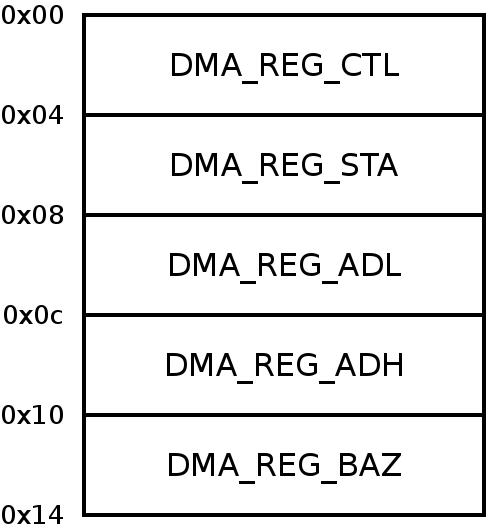
\includegraphics[scale=0.20]{../pic/dma_regs/main.jpeg}
\end{center}
\caption{\tiny{DMA registers}}
\label{dma_regs}
\end{figure}

\paragraph{}
Registers are described in the following sections.

\newpage
\subsection{DMA\_REG\_CTL}

\begin{figure}[!h]
\begin{center}
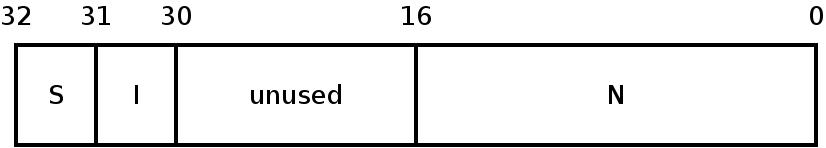
\includegraphics[scale=0.20]{../pic/dma_reg_ctl/main.jpeg}
\end{center}
\caption{\tiny{DMA control register}}
\label{dma_reg_ctl}
\end{figure}

\begin{table}[!h]
\centering
\begin{scriptsize}
\begin{tabular}{|p{1cm}|p{12cm}|}
  \hline
  \textit{name} & \textit{description} \\
  \hline
  S
  &
  set to 1 to start the transfer. self clears. \\
  \hline
  I
  &
  set to 1 to enable interrupt at end of transfer. default to 0. \\
  \hline
  N
  &
  size of the transfer, in bytes. \\
  \hline
\end{tabular}
\end{scriptsize}
\caption{\tiny{DMA\_REG\_CTL RW register fields}}
\label{tab:dma_reg_ctl_fields}
\end{table}

\newpage
\subsection{DMA\_REG\_STA}

\begin{figure}[!h]
\begin{center}
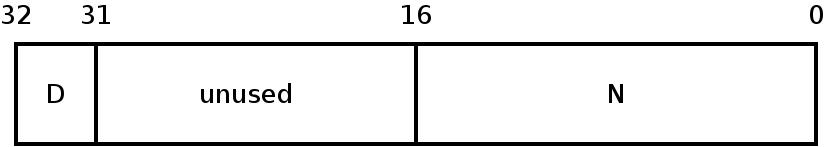
\includegraphics[scale=0.20]{../pic/dma_reg_sta/main.jpeg}
\end{center}
\caption{\tiny{DMA status register}}
\label{dma_reg_sta}
\end{figure}

\begin{table}[!h]
\centering
\begin{scriptsize}
\begin{tabular}{|p{1cm}|p{12cm}|}
  \hline
  \textit{name} & \textit{description} \\
  \hline
  D
  &
  automatically set to 1 when a transfer is done. 0 if a transfer is running.\\
  \hline
  N
  &
  size (in bytes) actually transfered. valid only when DMA not running (ie. R cleared). \\
  \hline
\end{tabular}
\end{scriptsize}
\caption{\tiny{DMA\_REG\_STA RO register fields}}
\label{tab:dma_reg_sta_fields}
\end{table}

\newpage
\subsection{DMA\_REG\_ADx}

\begin{figure}[!h]
\begin{center}
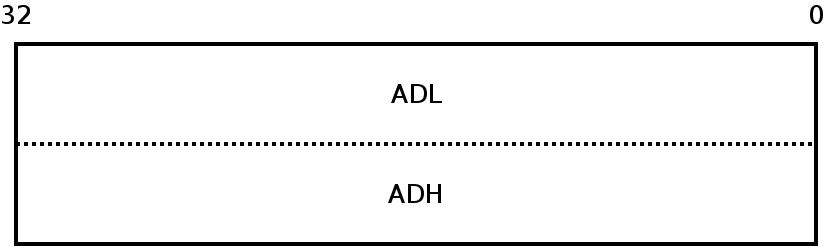
\includegraphics[scale=0.20]{../pic/dma_reg_adx/main.jpeg}
\end{center}
\caption{\tiny{DMA destination address register}}
\label{dma_reg_adx}
\end{figure}

\begin{table}[!h]
\centering
\begin{scriptsize}
\begin{tabular}{|p{1cm}|p{12cm}|}
  \hline
  \textit{name} & \textit{description} \\
  \hline
  ADL
  &
  destination address low part (32 least significant bits). \\
  \hline
  ADH
  &
  destination address high part (32 most significant bits). \\
  \hline
\end{tabular}
\end{scriptsize}
\caption{\tiny{DMA\_REG\_ADX RW register fields}}
\label{tab:dma_reg_adx_fields}
\end{table}

\newpage
\subsection{DMA\_REG\_BAZ}

\begin{figure}[!h]
\begin{center}
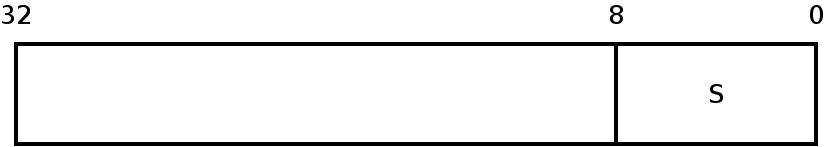
\includegraphics[scale=0.20]{../pic/dma_reg_baz/main.jpeg}
\end{center}
\caption{\tiny{DMA seed register}}
\label{dma_reg_baz}
\end{figure}

\begin{table}[!h]
\centering
\begin{scriptsize}
\begin{tabular}{|p{1cm}|p{12cm}|}
  \hline
  \textit{name} & \textit{description} \\
  \hline
  S
  &
  the user provided seed. default to 0. \\
  \hline
\end{tabular}
\end{scriptsize}
\caption{\tiny{DMA\_REG\_BAZ RW register fields}}
\label{tab:dma_reg_baz_fields}
\end{table}


%%
\newpage
\section{Application notes}

\subsection{Programming procedure}
\paragraph{}
When programming the DMA to perform a memory transfer, a user is expected to
follow this procedure:
\begin{enumerate}
\item the user eventually sets a seed in DMA\_REG\_BAZ[7:0],
\item the user sets DMA\_REG\_ADx with the 64 bits destination address,
\item the user sets DMA\_REG\_CTL[15:0] with the byte count to transfer,
\item the user eventually sets the DMA\_REG\_CTL I bit if an interrupt is
required at the end of the transfer,
\item the user sets the DMA\_REG\_CTL S bit to start the transfer,
\item the DMA set the DMA\_REG\_STA D bit upon transfer completion. An interrupt
is generated as indicated by the user,
\item the user reads the byte count actually transfered in the DMA\_REG\_STA
N field.
\end{enumerate}

\end{document}
